\documentclass{CInf_practice}

\sheet{6}{Flipflops und Registerschaltungen}

\begin{document}
\cinftitle

\ex{Zweiflankensteuerung}{5 + 7 = 12}
\begin{center}
  \noindent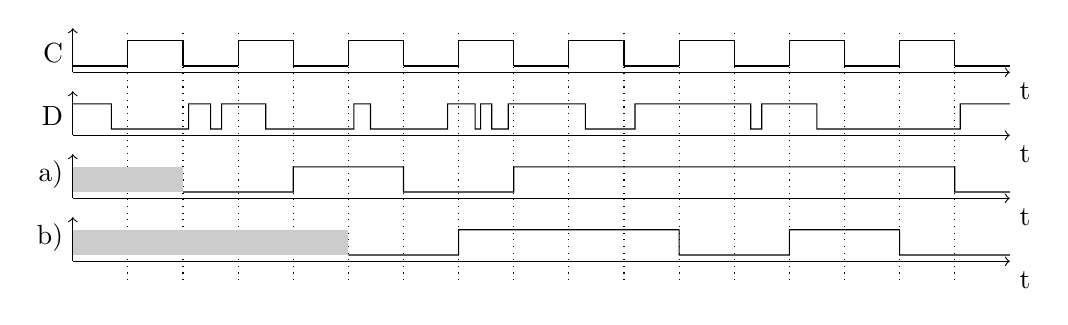
\begin{tikzpicture}[xscale=.7, yscale=.8]

    % helpers
    \def\hAzero{1.4}  \def\hAone{1.8}
    \def\hBzero{0.4}  \def\hBone{0.8}
    \def\hCyzero{3.4} \def\hCyone{3.8}
    \def\hDzero{2.4}  \def\hDone{2.8}

    \def\diff{.4}

    % undefs
    \def\drawundef#1#2{\fill[gray!40] (0, #1) rectangle ++(#2, -\diff);}

    % grid
    \foreach \name/\y in {C/4,D/3,a)/2,b)/1}{
      \draw[<-] (0,\y) -- ++(0,-.7) node[anchor=south east] {\name};
    }
    \foreach \y in {.3,1.3,2.3,3.3}{
      \draw[->] (0,\y) -- ++(17,0) node[anchor=north west] {t};
    }
    \foreach \x in {1,...,16}{
      \draw[dotted] (\x, 0) -- ++(0,4);
    }

    % draw helpers
    \def\drawAt#1#2{\draw (#1,#2) -- ++(1,0);}
    \def\connect#1#2{\draw (#2,#1) -- ++(0,\diff);}

    % draw cycle
    \foreach \x in {0,2,...,16}{
      \drawAt{\x}{\hCyzero}
      \connect{\hCyzero}{\x}
    }
    \foreach \x in {1,3,...,16}{
      \drawAt{\x}{\hCyone}
      \connect{\hCyzero}{\x}
    }

    % draw D
    \def\up{, \hDzero) -- ++(0, \diff) -- (}
    \def\dn{, \hDone)  -- ++(0, -\diff) -- (}
    \draw (0, \hDone) -- (.7 \dn 2.1 \up 2.5 \dn 2.7 \up 3.5 \dn 5.1 \up 5.4 \dn 
                         6.8 \up 7.3 \dn 7.4 \up 7.6 \dn 7.9 \up 9.3 \dn 10.2 \up
                         12.3 \dn 12.5 \up 13.5 \dn 16.1 \up 17, \hDone);

    % draw A
    \def\up{, \hAzero) |- ++(0, \diff) -- (}
    \def\dn{, \hAone)  -- ++(0, -\diff) -- (}
    \drawundef{\hAone}{2}
    \draw (2, \hAzero) -- (4 \up 6 \dn 8 \up 16 \dn 17, \hAzero);

    % draw B
    \def\up{, \hBzero) -- ++(0, \diff) -- (}
    \def\dn{, \hBone)  -- ++(0, -\diff) -- (}
    \drawundef{\hBone}{5}
    \draw (5, \hBzero) -- (7 \up 11 \dn 13 \up 15 \dn 17, \hBzero);

  \end{tikzpicture}
\end{center}

\ex{JK-Flipflops}{6 + 6 + 6 = 18}
\begin{center}
  \noindent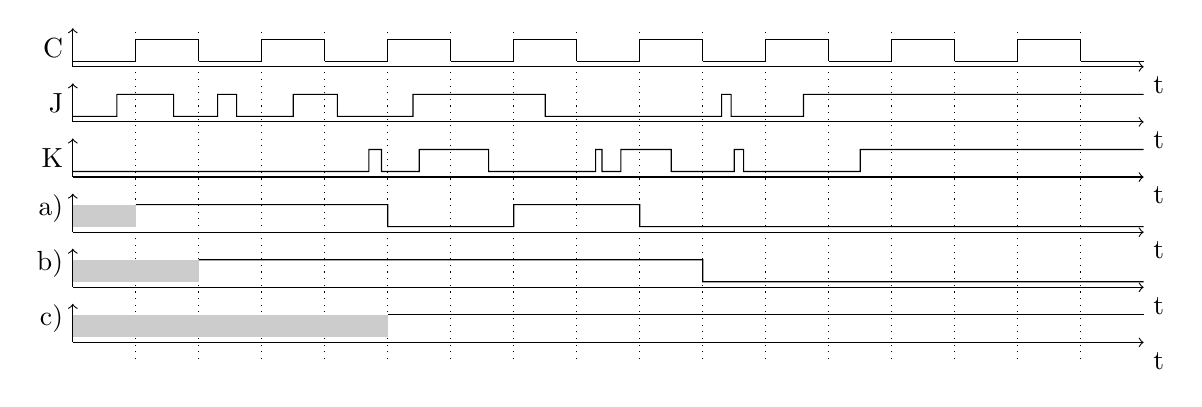
\begin{tikzpicture}[xscale=.8,yscale=.7]

    % helpers
    \def\hAzero{2.4}  \def\hAone{2.8}
    \def\hBzero{1.4}  \def\hBone{1.8}
    \def\hCzero{0.4}  \def\hCone{0.8}
    \def\hCyzero{5.4} \def\hCyone{5.8}
    \def\hJzero{4.4}  \def\hJone{4.8}
    \def\hKzero{3.4}  \def\hKone{3.8}

    \def\diff{.4}

    % undefs
    \def\drawundef#1#2{\fill[gray!40] (0, #1) rectangle ++(#2, -\diff);}
    

    % grid
    \foreach \name/\y in {C/6,J/5,K/4,a)/3,b)/2,c)/1}{
      \draw[<-] (0,\y) -- ++(0,-.7) node[anchor=south east] {\name};
    }
    \foreach \y in {.3,1.3,2.3,3.3,4.3,5.3}{
      \draw[->] (0,\y) -- ++(17,0) node[anchor=north west] {t};
    }
    \foreach \x in {1,...,16}{
      \draw[dotted] (\x, 0) -- ++(0,6);
    }

    % draw cycle
    \def\drawAt#1#2{\draw (#1,#2) -- ++(1,0);}
    \def\connect#1#2{\draw (#2,#1) -- ++(0,\diff);}
    \foreach \x in {0,2,...,16}{
      \drawAt{\x}{\hCyzero}
      \connect{\hCyzero}{\x}
    }
    \foreach \x in {1,3,...,16}{
      \drawAt{\x}{\hCyone}
      \connect{\hCyzero}{\x}
    }

    % draw J
    \def\up{, \hJzero) -- ++(0, \diff) -- (}
    \def\dn{, \hJone)  -- ++(0, -\diff) -- (}
    \draw (0, \hJzero) -- (.7 \up 1.6 \dn 2.3 \up 2.6 \dn 3.5 \up 4.2 \dn 
                          5.4 \up 7.5 \dn 10.3 \up 10.45 \dn 11.6 \up 
                          17, \hJone);
    
    % draw K
    \def\up{, \hKzero) -- ++(0, \diff) -- (}
    \def\dn{, \hKone)  -- ++(0, -\diff) -- (}
    \draw (0, \hKzero) -- (4.7 \up 4.9 \dn 5.5 \up 6.6 \dn 8.3 \up 8.4 \dn 
                           8.7 \up 9.5 \dn 10.5 \up 10.65 \dn 12.5 \up 
                           17, \hKone);

    % draw A
    \def\up{, \hAzero) |- ++(0, \diff) -- (}
    \def\dn{, \hAone)  -- ++(0, -\diff) -- (}
    \drawundef{\hAone}{1}
    \draw (1, \hAone) -- (5 \dn 7 \up 9 \dn 17, \hAzero);

    % draw B
    \def\up{, \hBzero) -- ++(0, \diff) -- (}
    \def\dn{, \hBone)  -- ++(0, -\diff) -- (}
    \drawundef{\hBone}{2}
    \draw (2, \hBone) -- (10 \dn 17, \hBzero);
    
    % draw C
    \def\up{, \hCzero) |- ++(0, \diff) -- (}
    \def\dn{, \hCone)  -- ++(0, -\diff) -- (}
    \drawundef{\hCone}{5}
    \draw (5, \hCone) -- (17, \hCone);
    
  \end{tikzpicture}
\end{center}


\end{document}
